% !TeX spellcheck = en_US

\chapter{Infrastructural code generation}
\label{chap: Code generation}
\section{Introduction}
After designing an OBSW model using the OSRA SCM model editor and following the component-based software development approach that comes with it, the OBSW model entities need to be mapped to the infrastructure code. The reference programming model for OSRA, discussed in the previous chapter helps us in progressing towards this goal. But, it is necessary to understand the overall design approach for the generated code and briefly present the abstractions that will be offered to the software supplier. This chapter, deals with these things in detail. Similar efforts from the Artemis JU CHESS project \cite{EvoRAVCodeAr}, provide the perfect base for discussions in this chapter of the Master thesis.   

\section{User model entities in the Platform Independent Model (PIM) phase}
A detailed description of all the modeling entities that the software architect can use, can be found in the specification of the metamodel for the OSRA component model \cite{SpecMetamodel}. However a brief description of them is noteworthy here:
 
\begin{description}
\item [Datatypes] The software architect can create a set of project-specific data types and constants using the \texttt{Data Types} language unit of the \texttt{CommonTypes} metamodel and the language unit is designed to provide the software architect an expressive power comparable to the languages with strong types (e.g. Ada).\cite{SpecMetamodel}. The supported type definitions are boolean types, integer types, float types, enumeration types, fixed point types, array types, structured types, string types, union types, alias types, opaque types, external types and unconstrained types. Some of the data type definitions are obvious for readers with programming skills in typed languages such as Ada, C or C++. 

\item [Interfaces] An interface is a specification of coherent set of services and it represents the definition of a contract. An interface is defined independently of the entities implementing it (e.g. Component type). An interface may enlist declaration of operations, which are the functional services that shall be offered by the entities implementing it. The services include a name, set of ordered parameters and one or more exceptions that they might throw when things go wrong during the handling of the service. Parameters are typed with one of the types mentioned above and have a mode (\texttt{in, out} or \texttt{inout}). A component type may expose one or more interfaces and the same interface can be exposed by different component types. An interface may also contain the declaration of one or more interface attributes, which are the parameters that are accessible via the interface implementations.

\item [Component type] A component type is an entity which specifies the external interfaces of a software component and are defined in isolation and are used to declare relationships with the other components and system in general. It conforms to the principle of encapsulation and as a consequence, all the interactions with other components are performed exclusively via its explicitly declared interface. A component type usually encompasses:
\begin{itemize}
\item A list of provided interface ports
\item A list of required interface ports
\item A list of dataset emitter ports 
\item A list of dataset receiver ports
\item A list of event emitter ports
\item A list of event receiver ports 
\end{itemize}

\item [Component implementation] It is an entity that represents a concrete realization of a component type. It is functionally identical to the component type except that the source code is added to the component implementation and may also define number of component implementation attributes

\item [Component instance] It is an instantiation of a component implementation and hence contains all the instantiations of the structural features, such as provided and required interface ports. It also contains instantiation of all attributes (interface attributes, component type attributes and component implementation attributes). It is also the elementary deployment unit for the OBSW model \cite{SpecMetamodel}.        
\end{description}

\section{Mapping of design entities to the infrastructural code}
As the generated code should target the Tasking framework, which is the target computational model in this Master thesis and because the Tasking framework is written in C++, the following sections explains mapping of design entities to the infrastructure code that will be generated in C++.

On analyzing the specification of the metamodel for the OSRA component model \cite{SpecMetamodel}, it is clear that there are different corner cases that can arise during the construction of the OBSW models using OSRA component model and it is necessary that these corner cases are effectively handled in the software design for the infrastructural code. The following sections try to build an OBSW model keeping the the corners cases in mind and attempt to explain the overall design approach.

\subsection{Corner cases arising during the construction of OBSW model using OSRA component model}
The different corner cases which can arise are:

\begin{itemize}
\item Multiple provided interfaces which refer to the same interface type are promoted by the container of a component
\item Multiple required interfaces which refer to the same interface type are subsumed by the container of a component
\item Multiple interfaces provide exact same operations
\item Multiple implementations per component type
\end{itemize}

The first and second corner cases are handled in the following example. But, the other cases will be treated directly in the later section, which deals with the software design for the generated infrastructure code. 

\subsection{An example OBSW model}
Our simple OBSW model, yet effective to serve the intended purpose, is built as per the proposed component-based development approach explained in the section \cref{section: Design steps} in chapter \cref{chap: Software development process}. As already mentioned in that section, the component-based approach puts a lot of emphasis on the definition of component interfaces \cite{CompBasedProcess} and it is followed here as well. Components are built from scratch using newly defined interfaces. All model entities defined here are instantiations of the modeling entities specified in the metamodel \cite{SpecMetamodel}. The OBSW model is designed using the OSRA SCM model editor mentioned in the section \cref{section: OSRA editor} in chapter \cref{chap: Software development process}. The model entities from the OSRA SCM model editor can be exported as images and they are used in this sub-section for illustration purposes.

In this simple example, two simple components are designed. The first component requests for a service which can add two numbers and this service is implemented in the second component. Different non-functional properties, as explained later in this section, are strewn on the required and provided interfaces to make the already boring example, a bit more interesting and also to capture the first and second corner cases in the example.

\begin{description}
\item [Step 1: Definition of data types and events] As the Master thesis requires to emphasize more on effectively capturing interactions and concurrency semantics required for communication between the designed components, the data types chosen in this example are fairly simple. But it is important to note that the scheme of mapping of these simple data types to the infrastructural code (explained in the later sections), can be scaled to fairly complex data types as well. The data types, exception types and the event type used in this example are as shown in \cref{fig: Ex. Datatypes etc.}  

\begin{itemize}
\item Two data types namely \texttt{Fixed\allowbreak Length\allowbreak String\allowbreak Type} and \texttt{Integer\allowbreak Type} of type \texttt{UNSIGNED} are defined and they are named as \texttt{StringType} and \texttt{IntegerType} respectively

\item Three exception types, named as \texttt{OperandException}, \texttt{MemoryException} and \texttt{Overflow\allowbreak Exception} are defined 

\item An \texttt{Event} type, which can be used for asynchronous notifications \cite{SpecMetamodel} is instantiated and it is named as \texttt{FailureEvent}. Two event parameters are also instantiated as shown in \cref{fig: Ex. Datatypes etc.}

\end{itemize} 

\item [Step 2: Definition of interfaces] Two interface namely \texttt{InterfaceA} and \texttt{InterfaceB} are designed as shown in \cref{fig: Ex. Datatypes etc.}. \texttt{InterfaceA} has only one single operation by name \texttt{CallOperationAdd} and \texttt{InterfaceB} has an operation by name \texttt{OperationAdd} and an interface attribute of data type \texttt{IntegerType} and named as \texttt{m\_StatusValue}.  

\begin{itemize}
\item The operation \texttt{CallOperationAdd} is a parameterless operation and it is intended to be the service which can in turn request the service which can add two numbers.

\item The operation \texttt{OperationAdd} in \texttt{InterfaceB}, as the name suggests, is intended to be the service which can add two numbers, send back the results and raise a pre-defined exception if necessary. It has three operation parameters and can throw different exceptions as mentioned in \cref{fig: Ex. Datatypes etc.}. 

\item The interface attribute \texttt{m\_StatusValue} in \texttt{InterfaceB} is of type \texttt{CFG} and it indicates that the interface attribute is a configurable parameter \cite{SpecMetamodel}. As a result, two operations for the purpose of setting and getting the values of the interface attribute are defined.      
\end{itemize}

\begin{figure}[h]
	\centering
	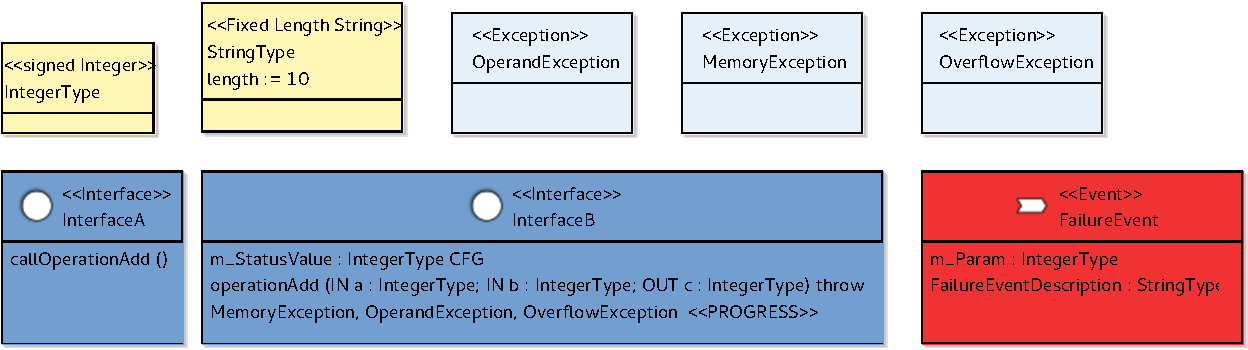
\includegraphics[width=1.0\textwidth]{InterfacesEventsDatasetsDiagram.pdf}
	\caption{Data types, events, exceptions and interfaces diagram}
	\label{fig: Ex. Datatypes etc.}
\end{figure}

\item [Step 3: Definition of component types] Component types namely \texttt{Component\allowbreak\_Caller} and \texttt{Component\allowbreak\_Callee} which form the basis for a reusable software asset are defined as shown in the \cref{fig: Ex. Component types}. 

\texttt{Component\allowbreak\_Caller} has:
\begin{itemize}
\item Provided interface port \texttt{Provided\allowbreak Interface\allowbreak Port} which refers to \texttt{InterfaceA}
\item Required interface port \texttt{Required\allowbreak Interface\allowbreak PortType1} which refers to \texttt{InterfaceB}
\item Required interface port \texttt{Required\allowbreak Interface\allowbreak PortType2} which refers to \texttt{InterfaceB}
\item Event receiver port \texttt{FailureEvent\allowbreak ReceiverPort} which refers to \texttt{Failure\allowbreak Event}
\end{itemize}

The desired interaction kind for the operations in the required interface ports of \texttt{Component\allowbreak\_Caller} are as shown in the table \cref{table: NFP RI Ports}

\begin{center}
\captionof{table}{Desired interaction kind for operations in the required interface ports} \label{table: NFP RI Ports} 
\begin{tabular}{|c|c|c|}
\hline
\thead{Required interface ports} & \thead{Operations} & \thead{Interaction kind} \\
\hline\hline
\texttt{Required\allowbreak Interface\allowbreak PortType1} & \makecell{\texttt{OperationAdd} \\ Interface attribute setter \\ Interface attribute getter} & \makecell{\texttt{synchronous} \\ \texttt{synchronous} \\ \texttt{synchronous}} \\
\hline
\texttt{Required\allowbreak Interface\allowbreak PortType2} & \makecell{\texttt{OperationAdd} \\ Interface attribute setter \\ Interface attribute getter} & \makecell{\texttt{asynchronous} \\ \texttt{asynchronous} \\ \texttt{asynchronous}} \\
\hline
\end{tabular}
\end{center}

\texttt{Component\allowbreak\_Callee} has:
\begin{itemize}
\item Provided interface port \texttt{Provided\allowbreak Interface\allowbreak Port1} which refers to \texttt{InterfaceB}
\item Provided interface port \texttt{Provided\allowbreak Interface\allowbreak Port2} which refers to \texttt{InterfaceB}
\item Event emitter port \texttt{FailureEvent\allowbreak EmitterPort} which refers to \texttt{FailureEvent}
\end{itemize}

\begin{figure}[h]
	\centering
	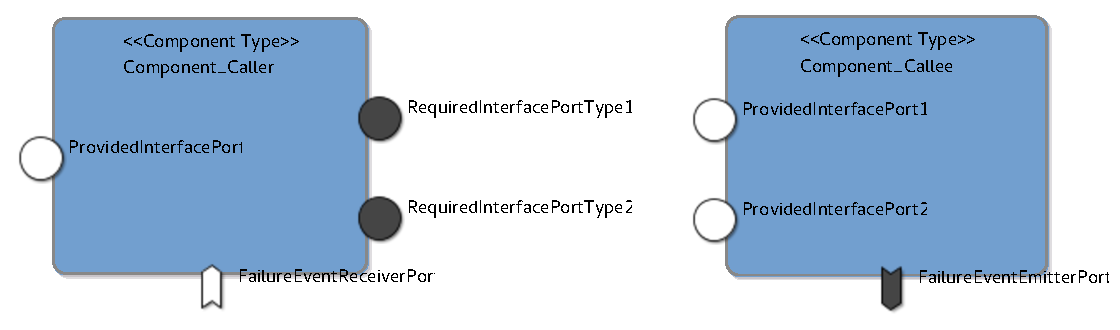
\includegraphics[width=1.0\textwidth]{ComponentTypesDiagram.pdf}
	\caption{Component types diagram}
	\label{fig: Ex. Component types}
\end{figure}

\item [Step 4: Definition of component implementations] Component implementations are created from the component types.

\texttt{Component\allowbreak\_Caller} has one component implementation named as \texttt{Component\allowbreak\_Caller\_impl} and \texttt{Component\allowbreak\_Callee} has one component implementation named as \texttt{Component\allowbreak\_Callee\_impl}. The component implementation \texttt{Component\allowbreak\_Callee\_impl} implements the means to store the attribute \texttt{m\_Param} of \texttt{InterfaceB}, that is exposed through its provided interface ports, namely \texttt{Provided\allowbreak Interface\allowbreak Port1} and \texttt{Provided\allowbreak Interface\allowbreak Port2}.

No maximum memory footprint for component implementations are defined or no detailed design activity of the component implementations are performed as they are not of concern in this Master thesis.

\item [Step 5: Definition of component instances] The component instances are the instances of component implementations \cite{CompBasedProcess}.

Two component instances as shown in \cref{fig: Ex. Component instances} are defined, namely:
\begin{itemize}
\item \texttt{Component\allowbreak\_Caller\_impl\_inst} which is an instantiation of \texttt{Component\allowbreak\_Caller\_impl}
\item \texttt{Component\allowbreak\_Callee\_impl\_inst} which is an instantiation of \texttt{Component\allowbreak\_Callee\_impl}
\end{itemize}

\item [Step 6: Definition of component bindings] Component bindings as shown in \cref{fig: Ex. Component instances} are defined:

\begin{figure}[h]
	\centering
	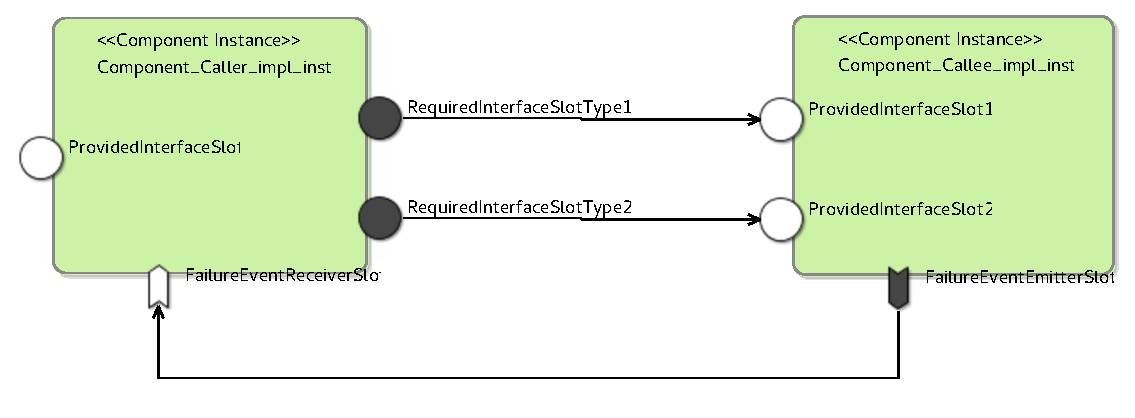
\includegraphics[width=1.0\textwidth]{ComponentInstancesDiagram.pdf}
	\caption{Component instances diagram}
	\label{fig: Ex. Component instances}
\end{figure}

\item [Step 7: Specification of non-functional attributes] The non-functional properties are defined on the component instances and the component bindings defined in the previous step. The non-functional properties language unit of the specification of a metamodel provides a Value Specification Language (VSL) unit, which permits the specification of the the non-functional properties qualified with a measurement unit \cite{SpecMetamodel}. VSL is used here to define values of non-functional properties with a measurement unit.

For the provided interface slot in the component instance \texttt{Component\allowbreak\_caller\_impl\_inst}, the following non-functional property is specified as shown in \cref{table: NFP PI Ports1}

\begin{center}
\captionof{table}{Non-functional property for the operation in the provided interface slot} \label{table: NFP PI Ports1}
\begin{tabular}{|c|c|c|}
\hline	
\thead{Provided interface slot} & \thead{Operation} & \thead{Non-functional property} \\
\hline \hline
\texttt{ProvidedInterface\allowbreak Slot} & \texttt{Call\allowbreak OperationAdd} & \makecell{\texttt{Cyclic}, Period = 2s} \\
\hline
\end{tabular}
\end{center}

For the provided interface slots in the component instance \texttt{Component\allowbreak\_callee\_impl\_inst}, the following non-functional properties are specified as shown in \cref{table: NFP PI Ports2}

\begin{center}
\captionof{table}{Non-functional properties for the operations in the provided interface slots} \label{table: NFP PI Ports2}
\begin{tabular}{|c|c|c|}
\hline	
\thead{Provided interface slots} & \thead{Operations} & \thead{Non-functional properties} \\
\hline \hline
\texttt{ProvidedInterface\allowbreak Slot1} & \makecell{\texttt{OperationAdd} \\ Interface attribute setter \\ Interface attribute getter} & \makecell{\texttt{Protected} \\ \texttt{Protected} \\ \texttt{Unprotected}} \\
\hline
\texttt{ProvidedInterface\allowbreak Slot2} & \makecell{\texttt{OperationAdd} \\ Interface attribute setter \\ Interface attribute getter} & \makecell{\texttt{Sporadic}, MIAT = 2s \\ \texttt{Protected} \\ \texttt{Protected}} \\
\hline
\end{tabular}
\end{center}

It is important to note that the WCET and deadline values for the operations in the provided interface slots are not handled, as the safeguarding of these properties are not of concern in this Master thesis.

For the event receiver slot in the component instance \texttt{Component\allowbreak\_caller\_impl\_inst}, the following non-functional property is specified as shown in \cref{table: NFP ER Port}

\begin{center}
\captionof{table}{Non-functional property for event reception} \label{table: NFP ER Port}
\begin{tabular}{|c|c|c|}
\hline	
\thead{Event receiver slot} & \thead{Event} & \thead{Non-functional property} \\
\hline \hline
\texttt{FailureEvent\allowbreak ReceiverSlot} & \texttt{FailureEvent} & \texttt{Protected} \\
\hline
\end{tabular}
\end{center}

\item [Step 8: Definition of the physical architecture] The hardware topology provides a description of the system hardware. As hardware modeling is not of concern of this Master thesis, a simple hardware topology as shown in \cref{fig: Ex. Hardware topology} is considered. 

A processor board with a processor and a processor core is instantiated. Two connection docks are attached to the processor board and a bus is used to connect the connection docks. The component instances are deployed on the processor core and the component bindings are deployed on the bus.

\begin{figure}[h]
	\centering
	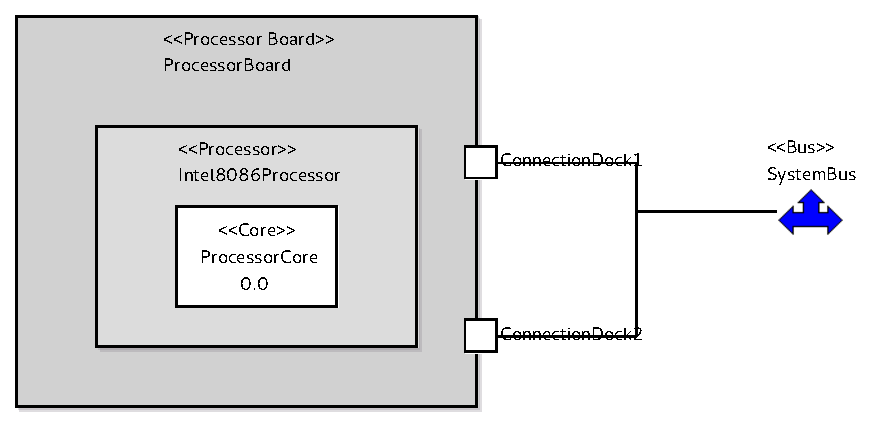
\includegraphics[width=0.8\textwidth]{HardwareDiagram.pdf}
	\caption{Hardware topology diagram}
	\label{fig: Ex. Hardware topology}
\end{figure}
 
\end{description}

This OBSW model is subjected to model validation against the OSRA Specification Compliance and the SCM meta-model compliance, in the OSRA SCM editor \cite{OSRAEditor}. Only after the OBSW model is successfully validated, can the OBSW model be considered as a suitable candidate for automatic generation of infrastructure code \cite{OSRAEditor}.  
   
\subsection{Software design approach for the generated code}
This section deals with the software design approach for the generated infrastructure code. UML class diagrams, wherever appropriate are judiciously used in this section to show a high level representation of the generated C++ classes. 

Each of the following sub-sections, is divided into two parts:
\begin{itemize}
\item The first part throws light on the idea of how a mapping of a given model entity to an infrastructural code entity can be done
\item The second part makes the approach clear by taking the reference of our OBSW example model discussed in the previous section  
\end{itemize}

\subsubsection{\textbf{Namespaces}}
Namespaces from C++ are used to differentiate component types, component implementations etc. of different components. The names for the namespaces are obtained from the names of the component types in the OBSW model.

\textbf{For our example OBSW model}: Three namespaces are created, namely \texttt{General}, \texttt{Component\_Caller} and \texttt{Component\_Callee} 

\subsubsection{\textbf{Data types and events}}
A data type from the OBSW model is translated into simple \texttt{typedef} statement from C++.

\textbf{For our example OBSW model}:
\begin{itemize}
\item The data type \texttt{IntegerType}, is translated to \texttt{typedef\allowbreak \ int8\_t IntegerType}
\item The data type \texttt{StringType}, is translated to \texttt{typedef\allowbreak \ std::string StringType} 
\end{itemize}

A subset of all possible data types from the OSRA Component Model can be translated to simple \texttt{typedef} statements as shown above. More information about the subset of data types for which this successfully works is given in the next chapter. 

The exception types from the OBSW models are translated into simple enumeration literals from C++. These exceptions, which can be thrown by a particular operation are grouped under an enumeration. This enumeration is further instantiated in a C++ struct.

\textbf{For our example OBSW model}: The three exceptions \texttt{Operand\allowbreak Exception}, \texttt{Memory\allowbreak Exception} and \texttt{Overflow\allowbreak Exception} are translated to enumeration literals. These exceptions can be thrown by \texttt{OperationAdd}, which is defined in \texttt{InterfaceB}. Hence the enumeration literals, corresponding to the exceptions, are stored together as an enumeration named \texttt{OperationAdd\allowbreak InterfaceB\allowbreak Exception} as shown in the \cref{fig: ExceptionsUML}. This exception is further instantiated in a C++ struct \texttt{OperationAdd\allowbreak InterfaceB\allowbreak Report} as shown in the \cref{fig: ExceptionsUML} 

\begin{figure}[h]
	\centering
	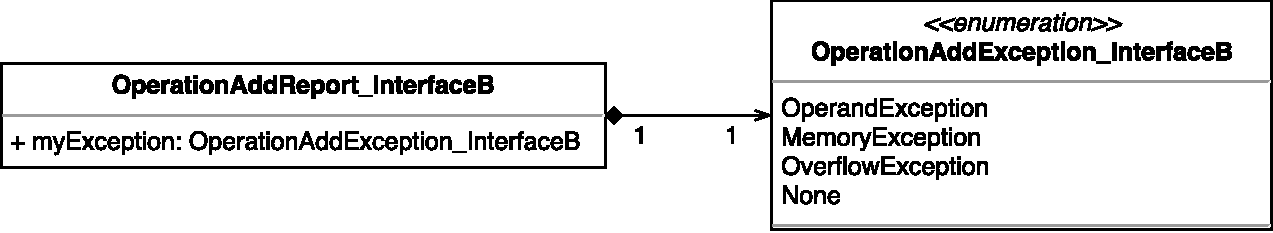
\includegraphics[width=0.8\textwidth]{ExceptionsUML.pdf}
	\caption{UML class diagram representation for exceptions in the example OBSW model}
	\label{fig: ExceptionsUML}
\end{figure}

An event from the OBSW model is mapped to an abstract base class and a corresponding concrete implementation class. Appropriate setters and getters for the event parameters are declared as pure virtual methods in the abstract base class for the event and they are implemented in their corresponding concrete implementation.

\textbf{For our example OBSW model}: The \texttt{FailureEvent} is mapped as an abstract base class named \texttt{FailureEvent\allowbreak Interface} and concrete implementation class named \texttt{FailureEvent}. Appropriate setters and getters for the event parameters \texttt{m\_Param} and \texttt{m\_ParamDescription} are declared as pure virtual methods in the \texttt{FailureEvent\allowbreak Interface} abstract base class and implemented in the \texttt{FailureEvent} concrete implementation class. An UML class diagram representation of the generated classes are as shown in \cref{fig: EventUML}.

\begin{figure}[h]
	\centering
	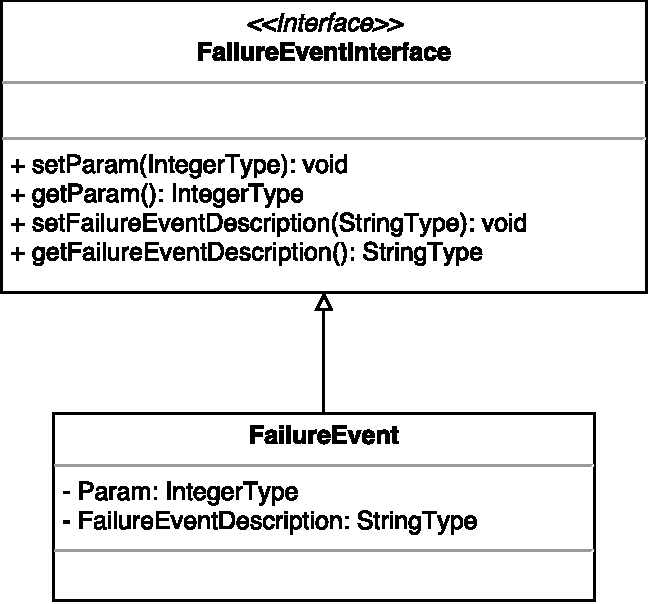
\includegraphics[width=0.4\textwidth]{EventUML.pdf}
	\caption{UML class diagram representation for event in the example OBSW model}
	\label{fig: EventUML}
\end{figure}    

All the infrastructure code entities mentioned above are present in a namespace, named as \texttt{General}.  

\subsubsection{\textbf{Interfaces}}
An interface can be mapped to an abstract base class in C++. Constituents of this abstract base class are:

\begin{itemize}
\item For each interface operation, corresponding operation parameters and corresponding data types of the operation parameters, a pure virtual method is declared. The names and data types of the input parameters for this pure virtual method corresponds to the names and data types of the interface operation parameters. The operation parameters, with \texttt{ParameterDirectionKind} as \texttt{in} are translated to constant references and the operation parameters with \texttt{ParameterDirectionKind} as \texttt{out} or \texttt{inout} are translated to plain references 
\item For each interface attribute parameter of type \texttt{CFG}:
\begin{itemize}
\item A class variable of name and data type corresponding to the name and data type of interface attribute is added
\item Pure virtual setter and getter methods for the interface attribute are declared. The data types and names of the input parameters in the setter and getter methods mimic the name and data type of the interface attribute.
\end{itemize} 
\item For each interface attribute parameter of type \texttt{MIS}, which is fixed once and for all and is not variable \cite{SpecMetamodel}: 
\begin{itemize}
\item A \texttt{const} class variable of name and data type corresponding to the name and data type of interface attribute is added
\item No getter and setter methods are added
\end{itemize}
\item For each interface attribute of type \texttt{DAT}, which are modifiable by the component only and not by external entities \cite{SpecMetamodel}:
\begin{itemize}
\item A class variable of name and data type corresponding to the name and data type of interface attribute is added
\item No getter and setter methods are added  
\end{itemize}   
\end{itemize}

\textbf{For our example OBSW model} The C++ classes shown in \cref{fig: InterfacesUML} are generated:
\begin{itemize}
\item \texttt{InterfaceA} along with the operation \texttt{CallOperationAdd} is mapped to an abstract base class \texttt{InterfaceA} with a pure virtual method \texttt{CallOperationAdd}. 
\item \texttt{InterfaceB} has one operation \texttt{OperationAdd} and one interface attribute parameter \texttt{m\_StatusValue} of type \texttt{CFG}. These are mapped to an abstract base class named \texttt{InterfaceB} with the following pure virtual methods:
\begin{itemize}
\item \texttt{OperationAdd} with two input parameters of type \texttt{const\allowbreak \ IntegerType\&} and one input parameter of type \texttt{IntegerType\&}
\item getter method for the interface attribute \texttt{m\_StatusValue} with an input parameter of type \texttt{IntegerType\&}
\item setter method for the interface attribute \texttt{m\_StatusValue} with an input parameter of type \texttt{const\allowbreak \ IntegerType\&}
\end{itemize} 
\end{itemize}

\begin{figure}[h]
	\centering
	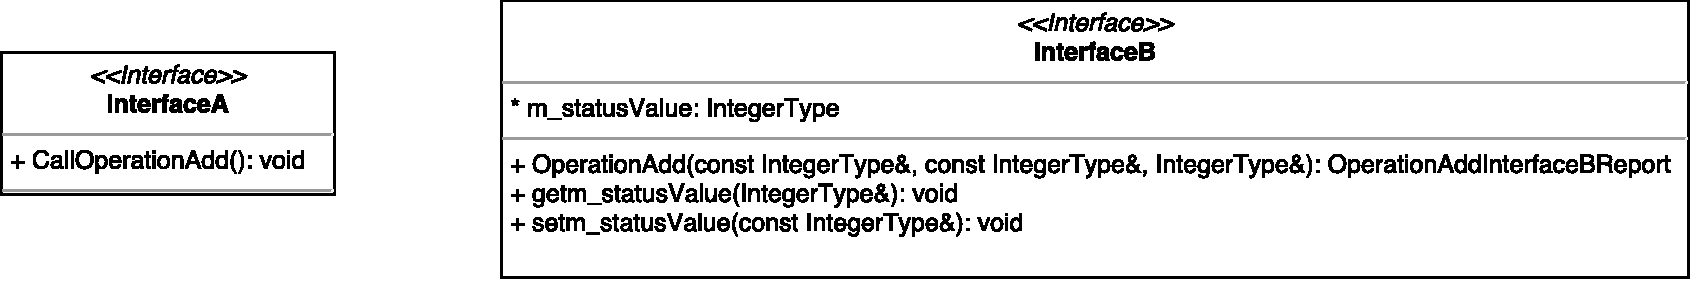
\includegraphics[width=0.8\textwidth]{InterfacesUML.pdf}
	\caption{UML class diagram representation for interfaces in the example OBSW model}
	\label{fig: InterfacesUML}
\end{figure}

Because of the corner case that multiple interfaces can have exactly same operations, it is necessary to refine these interfaces using the interface helper abstract base classes. In each interface helper class:
\begin{itemize}
\item Implementations for all the inherited pure virtual methods from the parent interface are provided
\item The implementation consist of simple method calls to new pure virtual methods
\item These new pure virtual methods have method signatures similar to the inherited and implemented pure virtual methods. However, it is important to note that the names of these new pure virtual methods are different from the inherited pure virtual methods
\item The implementation for the inherited pure virtual functions consist of a simple call to the newly declared pure virtual functions
\end{itemize}

\textbf{For our example OBSW model}:
\begin{itemize}
\item \texttt{InterfaceA\allowbreak\_Helper} is defined, which inherits from the interface \texttt{InterfaceA} and which implements the pure virtual method in the parent interface \texttt{InterfaceA}. The implementation contains a simple call to a new pure virtual method which has \texttt{\_InterfaceA} added to the original method name from the parent interface

\item \texttt{InterfaceB\allowbreak\_Helper} is defined, which inherits from the interface \texttt{InterfaceB} and which implements all the pure virtual methods in the parent interface \texttt{InterfaceB}. Each implementation contain a simple call to the new pure virtual methods which has \texttt{\_InterfaceB} added to the original method name from the parent interface    
\end{itemize}

The combined effect is that now, more than one original parent interfaces (resembling model entities) can have same operations. The refined interfaces redefine the methods from the original parent interfaces, so that there are no confusions between similar operations from different interfaces. Of course, a straight forward solution would have been to incorporate namespaces from C++, but it is not suitable for this design and the reason is explained later in this section. 

For each interface operation and interface attribute in an interface, a C++ struct is defined to carry around the values of the operation parameters or the values of the interface attributes. These data structures come in handy, when the interface operations or interface attribute access operations need to be accessed asynchronously. The data structures also hold general purpose polymorphic function wrappers from C++11 standard to store the call-back functions. 

\textbf{For our example OBSW model}:
\begin{itemize}
\item A struct \texttt{operationAdd\allowbreak Struct\_\allowbreak InterfaceB} is defined
\item A struct \texttt{statusValue\allowbreak Struct\_\allowbreak InterfaceB} is defined
\end{itemize}  

All the infrastructure code entities mentioned above are present in a namespace, named as \texttt{General}.

\subsubsection{\textbf{Parameter channels and parameter queues}}
The data structures which are defined to carry around the values of the operation parameters or values of the interface attributes, need to be put onto instances parameter channels, each one of which is supported in the back end by corresponding parameter queue.

\textbf{For all OBSW models}: \texttt{Parameter\allowbreak Channel} and \texttt{Parameter\allowbreak Queue} C++ classes are created.

All the infrastructure code entities mentioned above are present in a namespace, named as \texttt{General}.   

\subsubsection{\textbf{Event emitter ports and event receiver ports}}
The event emitter port for a particular event is mapped as an abstract base class and a corresponding concrete implementation class in C++. The event receiver port for a particular event is mapped only as an abstract base class.  

\textbf{For our example OBSW model}: The \texttt{FailureEvent\allowbreak EmitterPort} is mapped as a pair of abstract base class and a concrete implementation class. The abstract base class consists of a function that could be used by external actors to emit a \texttt{FailureEvent}.  

\textbf{For our example OBSW model}: The \texttt{FailureEvent\allowbreak ReceiverPort} is mapped as a pair of abstract base class and a concrete implementation class. The abstract base class consists of a method to receive the \texttt{FailureEvent} and it can be used by an external actor to send an event to the corresponding component.

The \texttt{FailureEvent\allowbreak EmitterPort} is present in a namespace, named as \texttt{Component\allowbreak\_Callee} and the \texttt{FailureEvent\texttt ReceiverPort} is present in a namespace, named as \texttt{Component\_Caller}. 

The \texttt{FailureEvent\allowbreak Emitter\allowbreak Port} is in namespace \texttt{Component\allowbreak \_Callee} and \texttt{FailureEvent\allowbreak Receiver\allowbreak Port} is in namespace \texttt{Component\allowbreak\_Caller}.

\subsubsection{\textbf{Component types}}
A component type can be mapped to an abstract base class in C++. A component type must provide all the operations that are listed in the provided interfaces of the component. Hence it inherits from all the interface helper classes which are referenced by its provided interfaces. This is where interface helper classes, with redefined operations come in handy, because C++ does not distinguish between operations with same signatures, although they are inherited from different namespaces. A component type must also inherit from the mapped abstract base classes for event receiver ports.

A component type must also have pure virtual methods which obtain and release the semaphores for the concurrent access of different operations that it provides. It must also provide pure virtual methods which are necessary to obtain and release semaphores meant for safely interleaving event receptions. In addition to these, pure virtual methods need to be added, which act as call-back functions for the operations, that the component type's required interface ports request to be released asynchronously.   

\textbf{For our example OBSW model}:
\begin{itemize}
\item \texttt{ComponentType} in the namespace \texttt{Component\_Caller} inherits from the \texttt{InterfaceA\allowbreak\_Helper} and also inherits from the abstract base class \texttt{FailureEvent\allowbreak ReceiverPort}. It has pure virtual methods meant for the purpose of obtaining and releasing of semaphores for concurrent accesses of the operation \texttt{CallOperationAdd\allowbreak\_InterfaceA} and reception of \texttt{FailureEvent}. It also has pure virtual methods which act as call-back functions, for the operation \texttt{OperationAdd}, for the getter operation of the interface attribute \texttt{m\_StatusValue} that the subsumed required interface port \texttt{RequiredInterfacePortType2} might request
\item \texttt{ComponentType} in the namespace \texttt{Component\_Callee} inherits from the \texttt{InterfaceB\allowbreak\_Helper}. It has pure virtual methods for the purpose of obtaining and releasing of semaphores for operations:
\begin{itemize}
\item {OperationAdd\allowbreak\_InterfaceB}
\item Setter and getter operations for the interface attribute \texttt{m\_StatusValue}
\end{itemize}   
\end{itemize}

\subsubsection{\textbf{Required interface ports}}
A required interface port is mapped as an abstract base class and a corresponding concrete implementation class in C++. The required interface subsumed by a particular component type has various operations that it might request and each operation has information whether the required interaction kind is \texttt{synchronous} pr \texttt{asynchronous} \cite{SpecMetamodel,CompBasedProcess}. Each required interface port refers to one interface and for each operation in the required interface port, a pure virtual method is added to the abstract base class. The signatures of these methods depend on whether the operations would be requested with an asynchronous release pattern or synchronous release pattern.

In case of interface operations:
\begin{itemize}
\item If the desired interaction kind for the operation is \texttt{synchronous}, then the signature of the method in the abstract base class is similar to the corresponding method in the abstract base class for the interface
\item If the desired interaction kind for the operation is \texttt{asynchronous}, then the signature of the method in the abstract base class is not similar to the corresponding method in the abstract base class for the interface. It is changed to replace the \texttt{out} and \texttt{inout} parameters with a single pointer to the respective call-back function in the corresponding abstract base class of its component type 
\end{itemize}

In case of interface attributes:
\begin{itemize}
\item For the setter of the interface attribute, signature of the method in the abstract class is similar to the corresponding method in the abstract based class for the interface
\item If the desired interaction kind for the getter of the interface attribute os \texttt{synchronous}, then the signature of the method in the abstract class is similar to the corresponding method in the abstract based class for the interface 
\item If the desired interaction kind for the getter of the interface attribute is \texttt{asynchronous}, then the signature of the method in the abstract base class is not similar to the corresponding method in the abstract base class for the interface. It is changed to replace the method parameter with a single pointer to the respective call-back function in the corresponding abstract base class of its component type  
\end{itemize} 

The concrete implementation for the methods is fairly simple, if the desired interaction kind for the corresponding operation is \texttt{synchronous}. The implementation consists of a simple method call to the corresponding operation in the abstract base class of the bound provided interface port.

The concrete implementation for the methods, in case the desired interaction kind for the corresponding operation is \texttt{asynchronous}, it would do the following things:
\begin{itemize}
\item Make local copies of all the method parameters
\item Pack them in the instances of data structures designed to carry the corresponding parameters
\item Simple method call to the corresponding operation in the abstract base class of the bound provided interface port
\end{itemize}            

\textbf{For our example OBSW model}: The following C++ classes are defined:
\begin{itemize}
\item \texttt{RequiredInterface\allowbreak PortType1Base} abstract base class and its corresponding \texttt{RequiredInterface\allowbreak Type1} concrete implementation class.
\item \texttt{RequiredInterface\allowbreak PortType2Base} abstract base class and its corresponding \texttt{RequiredInterface\allowbreak Type2} concrete implementation class
\end{itemize}

The \texttt{RequiredInterface\allowbreak PortType1Base} and \texttt{RequiredInterface\allowbreak PortType2Base} have pure virtual methods as per the general description and they have to implemented in the concrete implementation classes \texttt{RequiredInterface\allowbreak Type1} and \texttt{RequiredInterface\allowbreak Type2} respectively. The concrete implementations are in line with the description as in the general case above.

All the C++ classes mentioned above are present in the namespace \texttt{Component\allowbreak\_Caller}. As the component type \texttt{Component\allowbreak\_Callee} does not have any required interface ports, no C++ classes related to required interface ports are defined in the namespace \texttt{Component\allowbreak\_Callee}. 

\subsubsection{\textbf{Component implementations}}
A component implementation can be mapped in C++ as a concrete implementation of its abstract component type base class. It implements all the pure virtual methods that are inherited from its component type. It also has actual instances of semaphores for allowing safe concurrent accesses to the implemented methods and for safe interleaving between concurrent receptions of events of the same kind.

In case of components which promote multiple provided interface ports which refer to the same interface, it is necessary to provide multiple implementations for the operations in the provided interfaces. In order to solve this problem:
\begin{itemize}
\item A component implementation abstract base class is designed which contains implementations for inherited pure virtual methods related to acquiring and releasing of semaphores.
\item Component implementation abstract base class is further extended by dummy abstract base classes, one for each of the provided interface ports which refer to the same interface
\item These dummy abstract base classes are extended by concrete implementation classes which provide different concrete implementations for all the inherited operations except the ones, which are already implemented in the component implementation abstract base class
\item As it is a necessity to have only one instantiable concrete implementation per component, all the concrete implementations are inherited one last time in a component implementation class. This instance is now deployable on the hardware platform
\end{itemize}
 
\textbf{For our example OBSW model}:
\begin{itemize}
\item \texttt{Component\allowbreak Implementation} concrete implementation class in the namespace \texttt{Component\_Caller} inherits from the abstract base class \texttt{Component\_Type} in the same namespace. It implements all the pure virtual methods in the \texttt{ComponentType}.
\item Because the \texttt{ComponentType} in the namespace \texttt{Component\_Callee} has two provided interface ports namely, \texttt{Provided\allowbreak Interface\allowbreak Port1} and \texttt{Provided\allowbreak Interface\allowbreak Port2}, which refer to \texttt{InterfaceB}, the following classes are created:
\begin{itemize}
\item \texttt{ComponentImplementation\allowbreak Base} which is an abstract base class, but provides implementation for inherited pure virtual methods related to acquiring and releasing of semaphores
\item \texttt{Component\allowbreak Implementation\allowbreak Type1Base} and \texttt{Component\allowbreak Implementation\allowbreak Type2Base} which are dummy abstract base classes
\item \texttt{Component\allowbreak Implementation\allowbreak Type1} and \texttt{Component\allowbreak Implementation\allowbreak Type2} which provide different implementations for all the inherited operations except the ones implemented in \texttt{Component\allowbreak Implementation\allowbreak Base}
\end{itemize}   
\end{itemize} 

\subsubsection{\textbf{Provided interface ports}}
A provided interface port is mapped to an abstract base class and a corresponding concrete implementation class in C++. The provided interface promoted by a particular component type has various operations that are provided and each operation has information about the desired release pattern attached as a non-functional/extra-functional property \cite{SpecMetamodel,CompBasedProcess}. Each provided interface port refers to one interface and for each operation in the provided interface port, a pure virtual method is added to the abstract base class. The signatures of these methods depend on whether these operations are requested with a synchronous release pattern or an asynchronous release pattern.

In case of interface operations:
\begin{itemize}
\item If the interface operation on the provided interface is expected to be called synchronously, then the signature of the method in the abstract base class is similar to the corresponding method in the abstract base class for the interface
\item If the interface operation on the provided interface is expected to be called asynchronously, then the signature of the method in the abstract base class is changed to accept a data structure designed to carry the values of the parameters for the operation along with a function-wrapper for the call-back function, to which the results of the operation and exceptions (if any) need to be relayed back     
\end{itemize}   

In case of interface attributes:
\begin{itemize}
\item For the operations which set and get the values of the interface attributes synchronously, the signature of the methods in the abstract base class are similar to the corresponding method in the abstract base class for the interface
\item For an operation which set the value of the interface attributes asynchronously, the signature of the method in the abstract base class is changed to accept a data structure designed to carry the values of the interface attribute
\item For an operation which gets the value of the interface attributes asynchronously, the signature of the method in the abstract base class is changed to accept a data structure designed to carry the values of the interface attribute and a function-wrapper for the call-back function, to which the value of the interface attribute needs to be relayed back 
\end{itemize}

For each interface operation or interface attribute setter/getter operation, which is called asynchronously, an additional pure virtual method is declared in the abstract base class. This pure virtual method is used to store the address of the task channel, to which the data structure corresponding to the operation needs to be pushed.

The concrete implementation for the methods, in case the corresponding operation is requested to be released synchronously, consists of a simple call to the corresponding method in the referred interface. If the non-functional property attached with release of the operation on the provided interface side is \texttt{Protected}, then the implementation also includes acquiring and releasing of semaphore associated with the operation. For this, the methods in the corresponding component type are used 

The concrete implementation for the methods, in case the corresponding operation is requested to be released asynchronously, consist of pushing the data structure associated with the operation onto the corresponding task channel. 

\textbf{For our example OBSW model}: The following classes are defined:
\begin{itemize}
\item \texttt{Provided\allowbreak Interface1\allowbreak Base} abstract base class and its corresponding \texttt{Provided\allowbreak Interface\allowbreak Port1} concrete implementation class
\item \texttt{Provided\allowbreak Interface2\allowbreak Base} abstract base class and its corresponding \texttt{Provided\allowbreak Interface\allowbreak Port2} concrete implementation class
\end{itemize} 

The \texttt{Provided\allowbreak Interface2\allowbreak Base} abstract base class has three additional pure virtual methods to store:
\begin{itemize}
\item The address of the task channel to which the data structure for the interface operation \texttt{OperationAdd} needs to be pushed
\item The address of the task channel to which the data structure for the getter operation of the interface attribute \texttt{m\_StatusValue} needs to be pushed
\item The address of the task channel to which the data structure for the setter operation of the interface attribute \texttt{m\_StatusValue} needs to be pushed
\end{itemize}

The \texttt{Provided\allowbreak Interface1\allowbreak Base} and \texttt{Provided\allowbreak Interface2\allowbreak Base} have pure virtual methods as per the general description and they have to implemented in the concrete implementation classes \texttt{Provided\allowbreak Interface\allowbreak Port1} and \texttt{Provided\allowbreak Interface\allowbreak Port2} respectively. The concrete implementations are in line with the description as in the general case above.

It is important to mention that the general structures of the thread of control to handle the different combinations of possible non-functional properties are already explained in the chapter on a programming model for OSRA \cref{chap: Progamming model}

\subsubsection{\textbf{Tasks from the Tasking framework}}
In the discussions about designing a programming model for OSRA, it was clear that the threads of control might contain tasks from the Tasking framework. Each task is mapped to an abstract base class and a concrete implementation class in C++. A task would have instances of the required task inputs, task event as per the required thread of control. Each task has a reference to the component type in order to invoke the actual operations which are represented as pure virtual methods in the component type.

\textbf{For our example OBSW model}: The following classes are defined:
\begin{itemize}
\item \texttt{Periodic\allowbreak TaskBase} abstract base class and \texttt{PeriodicTask} concrete implementation class for 
\end{itemize} 

\subsubsection{\textbf{Component containers}}
A container of a component can be mapped to a class in C++. The component instance, event emitter and receiver slots, required interface slots, instances of tasks from the Tasking framework reside inside a component container. The number of task instances inside a component container depend on the number of operations in the provided interface which would be released asynchronously. 

 
   



 


 
